\documentclass{report}
\usepackage[T1]{fontenc} % Fontes T1
\usepackage[utf8]{inputenc} % Input UTF8
\usepackage[backend=biber, style=ieee]{biblatex} % para usar bibliografia
\usepackage{csquotes}
\usepackage[portuguese]{babel} %Usar língua inglesa
\usepackage{blindtext} % Gerar texto automáticamente
\usepackage[printonlyused]{acronym}
\usepackage{hyperref} % para autoref
\usepackage{graphicx}
\usepackage{listings}
        \usepackage{color}
        \definecolor{dkgreen}{rgb}{0,0.6,0}
        \definecolor{gray}{rgb}{0.5,0.5,0.5}
        \definecolor{mauve}{rgb}{0.8,0,0.82}
        \lstset{frame=tb, language=python, aboveskip=3mm, belowskip=3mm, showstringspaces=false, columns=flexible, basicstyle={\small\ttfamily}, numbers=none, numberstyle=\tiny\color{gray}, keywordstyle=\color{blue}, commentstyle=\color{dkgreen}, stringstyle=\color{mauve}, breaklines=true, breakatwhitespace=true, tabsize=3}

\bibliography{bibliografia}


\begin{document}
%%
% Definições
%
\def\titulo{PROJETO 2 - PLANEAMENTO}
\def\data{17 de Maio de 2015}
\def\autores{Domingos Nunes, Dzianis Bartashevich, Francisco Cunha, Leonardo Oliveira}
\def\autorescontactos{dfsn@ua.pt, bartashevich@ua.pt, franciscomiguelcunha@ua.pt, leonardooliveira@ua.pt}
\def\versao{Versão 1.0}
\def\departamento{Departamento de Eletrónica, Telecomunicações e Informática}
\def\empresa{Universidade de Aveiro}
\def\logotipo{images/ua.pdf}
%
%% CAPA %%
%
\begin{titlepage}

\begin{center}
%
\vspace*{50mm}
%
{\Huge \titulo}\\ 
%
\vspace{10mm}
%
{\Large \empresa}\\
%
\vspace{10mm}
%
{\LARGE \autores}\\ 
%
%
\vspace{30mm}
%
\begin{figure}[h]
\center
\includegraphics{\logotipo}
\end{figure}
%
\vspace{20mm}
\end{center}
%
\begin{flushright}
\versao
\end{flushright}
\end{titlepage}

%
%
%%  Página de Título %%
%
%
\title{%
{\Huge\textbf{\titulo}}\\
{\Large \departamento\\ \empresa}
}
%
\author{%
    \autores \\
    \autorescontactos
}
%
\date{\data}
%
\maketitle
%%%%%%%%%%%%%%%%%%%%%%%%%%%%%%%%%%%%%%%%%%%
% RESUMO
%
%
\pagenumbering{roman}



\tableofcontents
\listoffigures


%%%%%%%%%%%%%%%%%%%%%%%%%%%%%%%
\clearpage
\pagenumbering{arabic}

%%%%%%%%%%%%%%%%%%%%%%%%%%%%%%%%
\chapter{Introdução}
\label{chap.introducao}
Este documento contém uma abordagem geral das etapas de realização do projeto 2 de Laboratórios de Informática, de acordo com o enunciado disponibilizado na plataforma \textit{moodle} da universidade \cite{moodle}.

Neste sentido, este documento está dividido em 7 capítulos. Depois desta introdução, no \autoref{chap.estrutura} é apresentada a estrutura das páginas \ac{html} necessárias à interação com a aplicação, no \autoref{chap.servidor} são referidos alguns aspetos sobre o servidor, no \autoref{chap.som}, são tratados os módulos necessários ao processamento e geração de ficheiros de som e no \autoref{chap.base} é apresentada a árvore da base de dados a ser criada. Já no \autoref{chap.fases}, estão presentes as datas planeadas para o desenvolvimento do projeto, assim como a distribuição de tarefas da fase inicial. Finalmente, no \autoref{chap.finais} são apresentadas algumas considerações finais.

%%%%%%%%%%%%%%%%%%%%%%%%%%%%%%%%
\chapter{Páginas Web}
\label{chap.estrutura}

Para este projeto decidimos optar por três páginas web, para tornar a aplicação menos sobrecarregada visualmente e mais interativa do ponto de vista do utilizador.

A página que nos aparece ao iniciar a aplicação chama-se "Adicionar música" (ver \autoref{music}), na qual vamos introduzir o código \ac{rtttl} da respetiva música na primeira caixa de texto e depois pressionamos o botão em baixo para podermos enviar o código para o servidor.

\begin{figure}[htp]
\centering
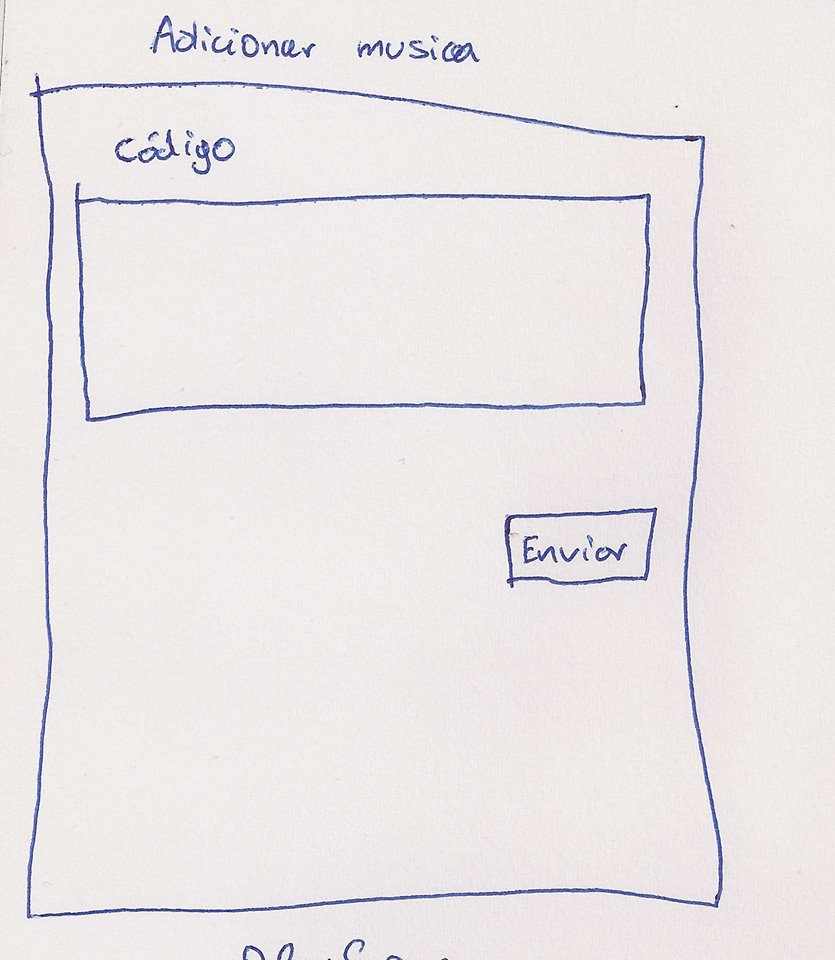
\includegraphics[width=\textwidth]{images/adicionarmusica.jpg}
\caption{Esboço da págna "Adicionar música".}
\label{music}
\end{figure}

Na página "Adicionar intepretação" (ver \autoref{inter}), como o nome indica, vamos adicionar uma nova intepretação a uma música. Temos um \textit{dropdown} que nos vai colocar em lista as músicas guardadas, uma caixa de texto para adicionarmos um registo e outro \textit{dropdown} para acrescentar um efeito à nossa escolha, como ilustra a figura. Após estas escolhas, temos de adicionar o nome que queremos dar à intepretação e enviar para o servidor.

\begin{figure}[htp]
\centering
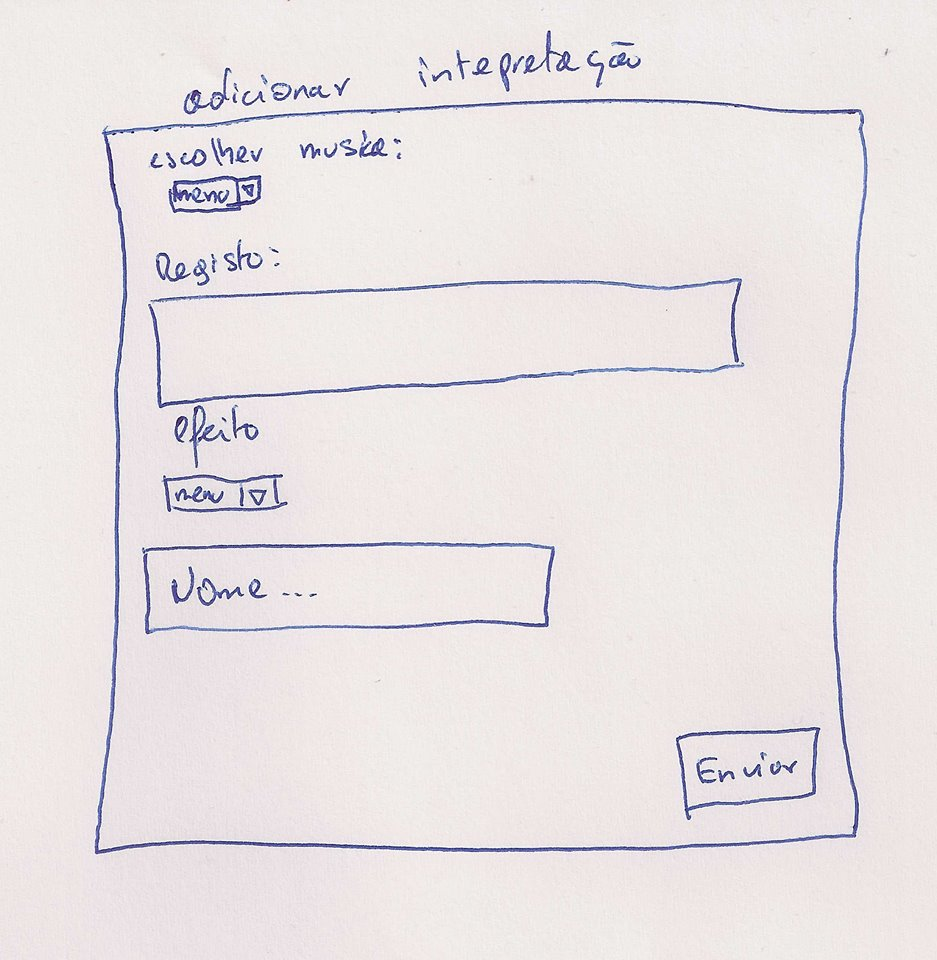
\includegraphics[width=\textwidth]{images/adicionarinterpretacao.jpg}
\caption{Esboço da págna "Adicionar interpretação".}
\label{inter}
\end{figure}

Finalmente, temos a página "Reproduzir música" (ver \autoref{play}), na qual vamos fazer essencialmente reproduzir música. Para isso temos de escolher a música num \textit{dropdown}, escolher a intepretação e carregar no \textit{play}. Ao lado de cada intepretação temos uma barra de gostos/não gostos para classificar cada música.

\begin{figure}[htp]
\centering
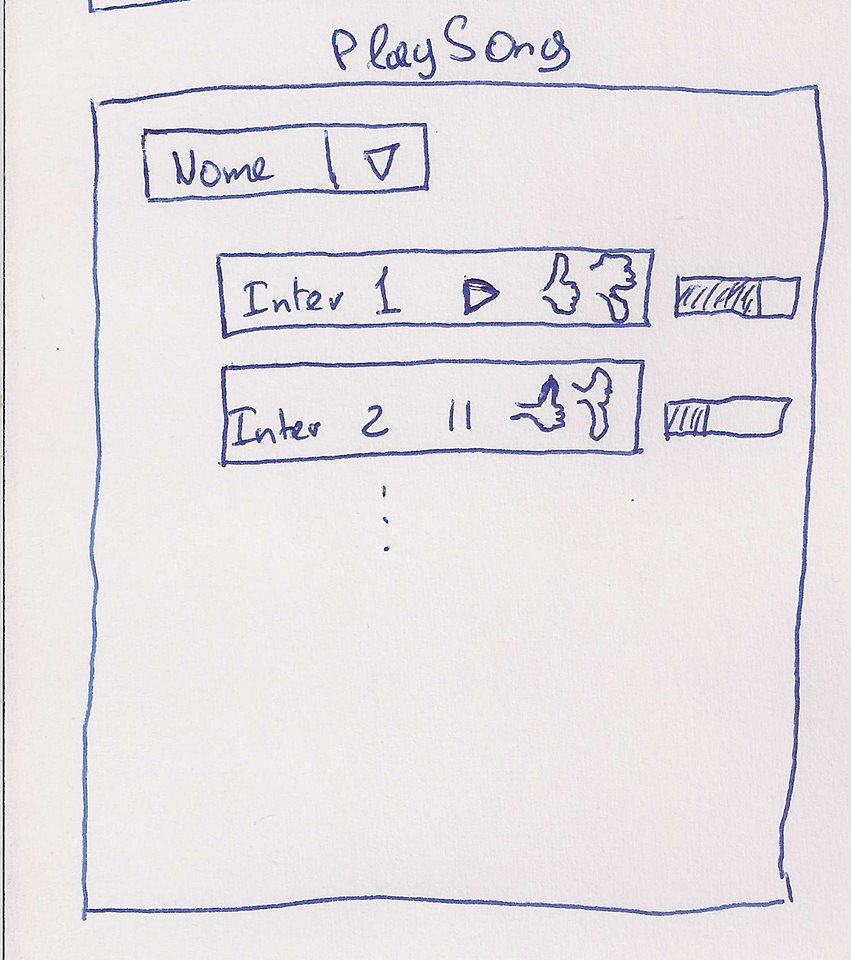
\includegraphics[width=\textwidth]{images/playsong.jpg}
\caption{Esboço da págna "Play song".}
\label{play}
\end{figure}

No decorrer do projeto vamos adicionar mais alguns botões e \textit{navbars} de modo a facilitar a navegação pela \textit{app}.


%%%%%%%%%%%%%%%%%%%%%%%%%%%%%%%%
\chapter{Servidor}
\label{chap.servidor}

Vai ser utilizado o módulo CherryPy \cite{cherry} para fazer um servidor HTTP que irá ter funcionalidades como GET e POST. Vai utilizar o \ac{json} como o meio de transporte de informação entre a base de dados e a Aplicação Web.

Os serviços a implementar seguirão o modelo dos colocados no enunciado do projeto.

Estamos a considerar não implementar o \emph{/getWaveFile} e \emph{/getWaveForm}, visto que, se guardarmos os ficheiros com o nome igual ao seu identificador, a sua procura é facilitada, podendo-se aceder diretamente ao \emph{link} em que se encontram. Por exemplo, para obter o ficheiro de música da interpretação com id 5, acedemos a \emph{/interpretations/5.wav}.

Se o utilziador pedir a lista de músicas existentes (\emph{/listSongs}), o servidor acede à base de dados e irá gerar um ficheiro \ac{json} com informação das músicas existentes e a aplicação web irá interpretar esse ficheiro. Um exemplo de ficheiro \ac{json} poderia ser:

\begin{lstlisting}
{
    {
        "id": 1,
        "name": "The Simpsons"
    },
    {
        "id": 2,
        "name": "The Family Guy"
    }
}
\end{lstlisting}

%%%%%%%%%%%%%%%%%%%%%%%%%%%%%%%%
\chapter{Som}
\label{chap.som}

Os módulos ligados ao processamento e geração de ficheiros de som seguirão os moldes do que foi sugerido no enunciado do projeto. Será criado um interpretador de pautas, um sintetizador e um processador de efeitos.

\chapter{Árvore da base de dados}
\label{chap.base}

A base de dados associada ao projecto serão duas tabelas \textbf{musics, interpretation} que estão interligadas entre si e as quais servirão para armazenar informação acerca dos conteúdos.
A tabela \textbf{musics} conterá informação com o \textbf{name} das músicas criadas e as \textbf{notes} (pautas) que lhes são correspondentes, sendo que a estes dois campos há um \textbf{id} que os identifica.

Por outro lado, a tabela \textbf{interpretation} terá campos como
\textbf{\texttt{id\_music}} que estará associado à tabela \textbf{musics}. Conterá também campos como \textbf{(registration)} (registos) que servirá para a codificação do registo  e o campo \textbf{effects} (efeitos), servindo para guardar informação sobre e os efeitos utilizados na música.
Finalmente, os campos \textbf{upvotes} e \textbf{downvotes} guardarão respectivamente o número de votos positivos e negativos. 


A \autoref{tree} apresenta o esquema da árvore da base de dados.

\begin{figure}[htp]
\centering
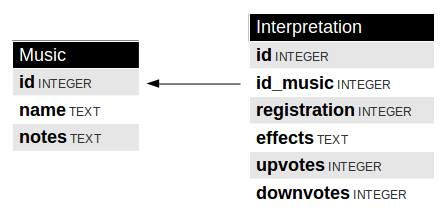
\includegraphics[width=\textwidth]{images/tree.jpg}
\caption{Árvore da base de dados, com as tabelas da música (\emph{musics}) e interpretação (\emph{interpretation}).}
\label{tree}
\end{figure}

%%%%%%%%%%%%%%%%%%%%%%%%%%%%%%%%
\chapter{Fases de desenvolvimento}
\label{chap.fases}
Estão previstas três fases de desenvolvimento do projeto:

\begin{itemize}
\item Fase 1 - 13 de Maio a 21 de Maio (a decorrer);
\item Fase 2 - 22 de Maio a 29 de Maio;
\item Fase 3 - 30 de Maio a 7 de Junho.
\end{itemize}

\section{Fase 1}
Inicialmente, será desenvolvida cada uma das partes da aplicação em separado e a distribuição das tarefas é a seguinte:
\begin{itemize}
\item Domingos - Implementação do \textit{mockup} das páginas \ac{html};
\item Dzianis - Implementação do servido;
\item Francisco - Implementação da base de dados;
\item Leonardo - Implementação do sintetizador e interpretador de pautas.
\end{itemize}
\section{Fase 2}
Neste fase a aplicação será testada no seu todo, sendo efetuados os ajustes necessários ao seu correto funcionamento, podendo ser acrescentadas algumas funcionalidades úteis que não tenham sido previstas.
\section{Fase 3}
Finalmente, serão afetuados os ajustes finais, sendo também completado o módulo processador de efeitos, para que este comece efetivamente a criar efeitos nas músicas: Echo, Tremolo, Distorção, Percursão, Chorus e Envelope.

%%%%%%%%%%%%%%%%%%%%%%%%%%%%%%%%
\chapter{Considerações finais}
\label{chap.finais}

As considerações feitas neste documento estão abertas a alterações, pelo que poderão ser efetuados ajustes nas funcionalidades implementadas ou na distribuição de tarefas caso seja necessário.

Embora não tenha sido aqui referido com pormenor, serão efetuados alguns testes (manuais e automáticos) a cada um dos componentes desenvolvidos e que serão, sempre que possível, da responsabilidade de um elemento que não tenha desenvolvido esse componente, para que seja mais ágil a deteção de erros e para que todos possamos ter uma melhor perseção do que foi feito pelos restantes colegas.


%%%%%%%%%%%%%%%%%%%%%%%%%%%%%%%%%
\chapter*{Acrónimos}
\begin{acronym}
\acro{sql}[SQL] {Structured Query Language}
\acro{html} [HTML] {HyperText Markup Language}
\acro{rtttl} [RTTTL] {Ring Tone Transfer Language}
\acro{json} [JSON] {JavaScript Object Notation}

\end{acronym}


%%%%%%%%%%%%%%%%%%%%%%%%%%%%%%%%%
\printbibliography

\end{document}